%\thispagestyle{myheadings}
\section{Keynote Address: Corinna Cortes}
\index{Cortes, Corinna}

\begin{center}

\begin{Large}
{\bfseries\Large ``Learning Ensembles of Structured Prediction Rules''}\vspace{1em}\par
\end{Large}

%% \begin{center}
%%   \begin{tabular}{m{1in}b{1in}}
%%     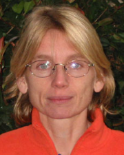
\includegraphics[width=1in]{content/monday/cortes-headshot.png}
%%     & {\bfseries Corinna Cortes} \newline Google Research, NY
%%   \end{tabular}
%% \end{center}

\daydateyear, 5:00--6:00pm \vspace{1em}\\
\PlenaryLoc \\
\vspace{1em}\par
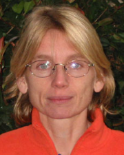
\includegraphics[height=100px]{content/monday/cortes-headshot.png}
\end{center}

\noindent
{\bfseries Abstract:} We present a series of algorithms with
theoretical guarantees for learning accurate ensembles of several
structured prediction rules for which no prior knowledge is assumed.
This includes a number of randomized and deterministic algorithms
devised by converting on-line learning algorithms to batch ones, and a
boosting-style algorithm applicable in the context of structured
prediction with a large number of labels. We also report the results
of extensive experiments with these algorithms.

This is joint work with Vitaly Kuznetsov, NYU, and Mehryar Mohri, NYU/Google
Research.

\vspace{3em}\par 

\vfill
\noindent

{\bfseries Biography:} Corinna Cortes is the Head of Google Research,
NY, where she is working on a broad range of theoretical and applied
large-scale machine learning problems. Prior to Google, Corinna spent
more than ten years at AT\&T Labs - Research, formerly AT\&T Bell Labs,
where she held a distinguished research position. Corinna's research
work is well-known in particular for her contributions to the
theoretical foundations of support vector machines (SVMs), for which
she jointly with Vladimir Vapnik received the 2008 Paris Kanellakis
Theory and Practice Award, and her work on data-mining in very large
data sets for which she was awarded the AT\&T Science and Technology
Medal in the year 2000. Corinna received her MS degree in Physics from
University of Copenhagen and joined AT\&T Bell Labs as a researcher in
1989. She received her Ph.D. in computer science from the University
of Rochester in 1993. Corinna is also a competitive runner.

\newpage
